\section{requirements engineering}\label{requirementsengineering}
Figure \ref{fig:useCaseDiagram} shows the use case diagram for ComeTogether.

\section{Design}\label{Design}

In figure \ref{fig:UserServiceREST} you can see the design for the UserService. UserServiceREST encapsulate the REST-Functionality of the UserService. UserPersistence access database with prepared statements p.e. to save, read or delete users. Between UserServiceREST and UserPersistence are service class and DAO class to encapsulate different levels of abstraction. Beside UserServiceREST there are the classes EventServiceREST, ParticipationServiceREST and MessageServiceREST. EventServiceREST in figure \ref{fig:EventServiceREST} creates, reads and deletes events. ParticipationServiceREST in figure \ref{fig:ParticipationServiceREST} creates participations and gives back a list of participation for a given eventid or a given userid. MessageServiceREST in figure \ref{fig:MessageServiceREST} creates, reads or deletes messages.

\begin{figure}[htp]
\centering
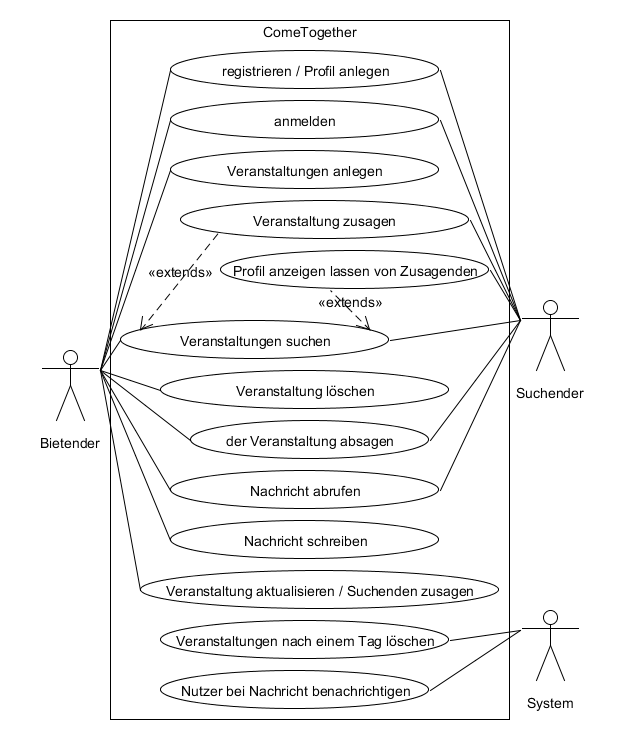
\includegraphics[width=0.5\textwidth]{Ingo/pictures/UseCaseDiagram.png}
\caption{use case diagram}
\label{fig:useCaseDiagram}
\end{figure}


\begin{figure}[htp]
\centering
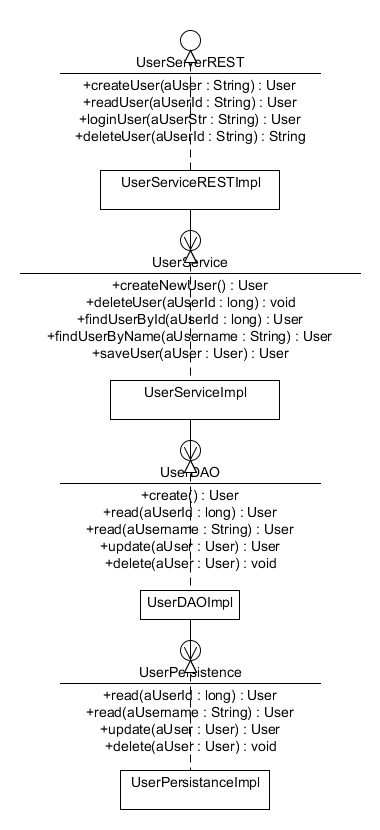
\includegraphics[width=0.5\textwidth]{Ingo/pictures/Design_User.png}
\caption{desing class diagramm UserServiceREST}
\label{fig:UserServiceREST}
\end{figure}


\begin{figure}[htp]
\centering
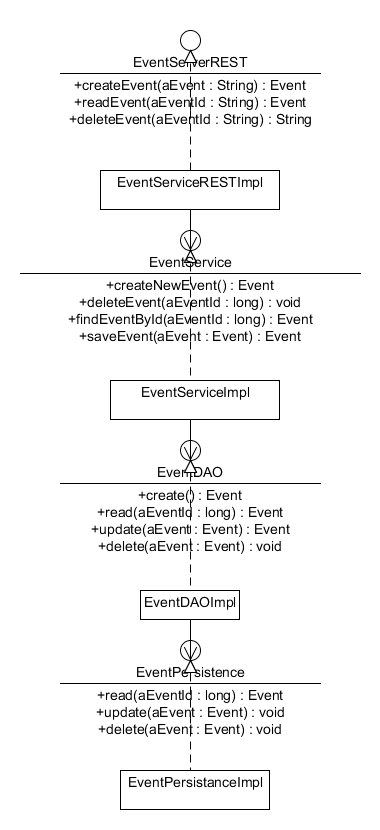
\includegraphics[width=0.5\textwidth]{Ingo/pictures/Design_Event.png}
\caption{desing class diagramm EventServiceREST}
\label{fig:EventServiceREST}
\end{figure}


\begin{figure}[htp]
\centering
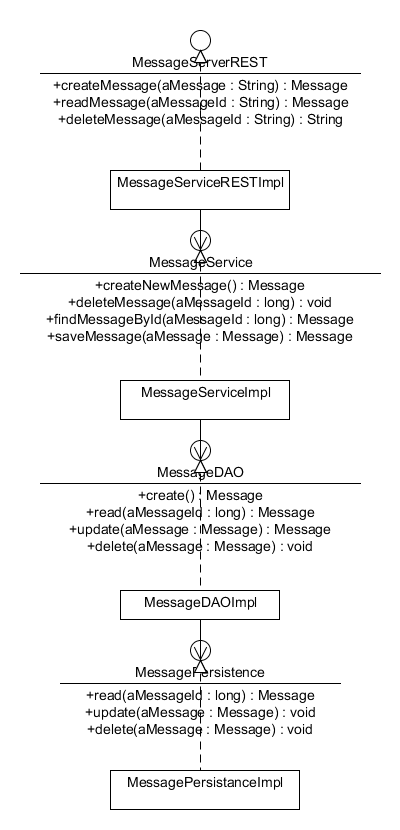
\includegraphics[width=0.5\textwidth]{Ingo/pictures/Design_Message.png}
\caption{desing class diagramm MessageServiceREST}
\label{fig:MessageServiceREST}
\end{figure}


\begin{figure}[htp]
\centering
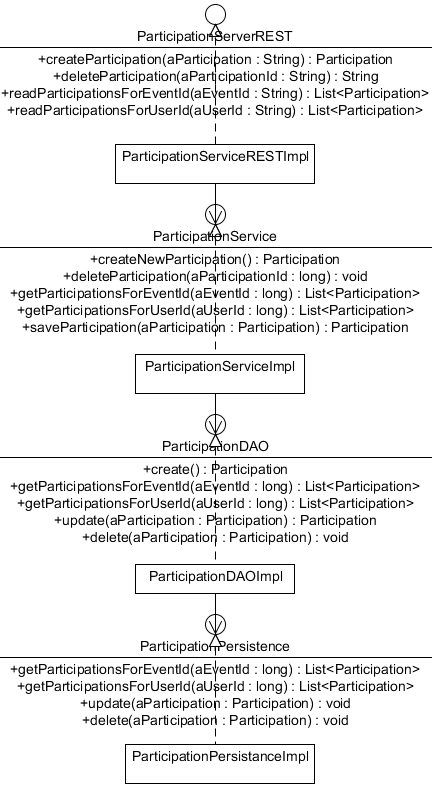
\includegraphics[width=0.5\textwidth]{Ingo/pictures/Design_Participation.png}
\caption{desing class diagramm ParticipationServiceREST}
\label{fig:ParticipationServiceREST}
\end{figure}
